\documentclass{standalone}
\usepackage{tikz}
\usetikzlibrary{patterns, angles}
\usepackage{circuitikz}

\begin{document}
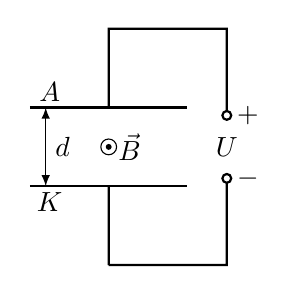
\begin{tikzpicture}[european] 
	\draw [thick] (1,0) -- (1,1)  (1,2) -- (1,3) -- (2.5,3) to [short, -o] (2.5,1.9) node [right] {$+$};
	\draw [thick] (1,0) -- (2.5,0) to [short, -o] (2.5, 1.1) node [right] {$-$};
	\node at (2.5,1.5) {$U$};
	\node at (1,1.5) [right] {$\vec{B}$};
	\draw (1,1.5) circle (0.1);
	\draw [fill] (1,1.5) circle (0.03);	
	\node at (0.25,2.2) {$A$};
	\node at (0.25,0.8) {$K$};
	\draw [arrows={latex-latex}] (0.2,1)--(0.2,2) node [midway, right] {$d$};
	\draw [thick] (0,1)--(2,1) (0,2)--(2,2);
\end{tikzpicture}
\end{document}